%%%%%%%%%%%%%%%%%%%%%%%%%%%%%%%%%%%%%%%%%
% Jacobs Landscape Poster
% LaTeX Template
% Version 1.0 (29/03/13)
%
% Created by:
% Computational Physics and Biophysics Group, Jacobs University
% https://teamwork.jacobs-university.de:8443/confluence/display/CoPandBiG/LaTeX+Poster
% 
% Further modified by:
% Nathaniel Johnston (nathaniel@njohnston.ca)
%
% This template has been downloaded from:
% http://www.LaTeXTemplates.com
%
% License:
% CC BY-NC-SA 3.0 (http://creativecommons.org/licenses/by-nc-sa/3.0/)
%
%%%%%%%%%%%%%%%%%%%%%%%%%%%%%%%%%%%%%%%%%

%----------------------------------------------------------------------------------------
%  PACKAGES AND OTHER DOCUMENT CONFIGURATIONS
%----------------------------------------------------------------------------------------

\documentclass[final]{beamer}

\usepackage[scale=1.24]{beamerposter} % Use the beamerposter package for laying out the poster
\usepackage{microtype}
\usepackage{cite}
\usepackage{multirow}
\usepackage{hhline}
\usepackage{enumerate}
\usepackage[english]{babel}
\usepackage{wrapfig}
\usepackage{float}
\usepackage{dcolumn}
\usepackage{sidecap}
%\usepackage{subcaption}

%% for row colors
\usepackage{xcolor,colortbl}
\definecolor{silver}{RGB}{192, 192, 192}

\usetheme{confposter} % Use the confposter theme supplied with this template

\setbeamercolor{block title}{fg=Maroon,bg=white} % Colors of the block titles
\setbeamercolor{block body}{fg=black,bg=white} % Colors of the body of blocks
\setbeamercolor{block alerted title}{fg=white,bg=Maroon} % Colors of the highlighted block titles
\setbeamercolor{block alerted body}{fg=black,bg=dblue!10} % Colors of the body of highlighted blocks
\setbeamerfont{block body}{family=\rmfamily,size={\fontsize{28}{32}}}
\setbeamerfont{block alerted body}{family=\rmfamily,size={\fontsize{28}{32}}}
\setbeamerfont{block alerted title}{family=\rmfamily,size={\fontsize{32}{36}}}
\setbeamerfont{block title}{family=\rmfamily,size={\fontsize{32}{36}}}
\setbeamerfont{title in headline}{family=\rmfamily,size={\fontsize{36}{40}}}
\setbeamerfont{itemize/enumerate body}{size={\fontsize{26}{32}}}
\setbeamerfont{itemize/enumerate subbody}{size={\fontsize{26}{32}}}
\selectfont
% Many more colors are available for use in beamerthemeconfposter.sty

%-----------------------------------------------------------
% Define the column widths and overall poster size
% To set effective sepwid, onecolwid and twocolwid values, first choose how many columns you want and how much separation you want between columns
% In this template, the separation width chosen is 0.024 of the paper width and a 4-column layout
% onecolwid should therefore be (1-(# of columns+1)*sepwid)/# of columns e.g. (1-(4+1)*0.024)/4 = 0.22
% Set twocolwid to be (2*onecolwid)+sepwid = 0.464
% Set threecolwid to be (3*onecolwid)+2*sepwid = 0.708

\newlength{\sepwid}
\newlength{\onecolwid}
\newlength{\twocolwid}
\newlength{\threecolwid}
\setlength{\paperwidth}{46.8in} % A0 width: 46.8in
\setlength{\paperheight}{33.1in} % A0 height: 33.1in
\setlength{\sepwid}{0.012\paperwidth} % Separation width (white space) between columns
\setlength{\onecolwid}{0.3\paperwidth} % Width of one column
%\setlength{\onecolwid}{0.235\paperwidth} % Width of one column
\setlength{\twocolwid}{0.482\paperwidth} % Width of two columns
\setlength{\threecolwid}{0.729\paperwidth} % Width of three columns
\setlength{\topmargin}{-0.5in} % Reduce the top margin size
% \setlength{\parindent}{1cm}
\newcommand{\tab}{\hspace*{1em}}
%-----------------------------------------------------------

\usepackage{graphicx}  % Required for including images

\usepackage{booktabs} % Top and bottom rules for tables

%----------------------------------------------------------------------------------------
%	TITLE SECTION 
%----------------------------------------------------------------------------------------


\title{Bayesian Hierarchical Reporting Delay Model in Infectious Disease Forecasting} % Poster title

%\author{\small Krzysztof Sakrejda$^\star$, Justin Lessler$^{\dagger}$, Nicholas Reich$^\star$} % Author(s)

%\institute{\tiny$^\star$University of Massachusetts - Amherst, $^\dagger$Johns Hopkins Bloomberg School of Public Health
%} % Institution(s)

\author{\small Krzysztof Sakrejda$^\star$, Nicholas Reich$^\star$, Stephen Lauer$^\star$, 
        Derek Cummings$^{\dagger,\ddagger}$, Paphanij Suangtho$^{\star\star}$, \\
        Soawapak Hinjoy$^{\star\star}$, Sopon Iamsirithaworn$^{\dagger\dagger}$, 
        Suthanun Suthachana$^{\star\star}$, 
        Hannah Clapham$^{\dagger}$, Justin Lessler$^{\dagger}$} % Author(s)

\institute{\tiny$^\star$University of Massachusetts - Amherst, $^\dagger$Johns Hopkins Bloomberg School of Public Health, 
           $^\ddagger$University of Florida, \\
           $^{\star\star}$Bureau of Epidemiology, Bangkok - Thailand,
           $^{\dagger\dagger}$Office of Disease Prevention and Control I - Bangkok,
           $^{\ddagger\ddagger}$Communicable Disease Section - Nonthaburi}

%----------------------------------------------------------------------------------------

\begin{document}
\addtobeamertemplate{block end}{}{\vspace*{2ex}} % White space under blocks
\addtobeamertemplate{block alerted end}{}{\vspace*{2ex}} % White space under highlighted (alert) blocks

\setlength{\belowcaptionskip}{2ex} % White space under figures
\setlength\belowdisplayshortskip{2ex} % White space under equations

\begin{frame}[t] % The whole poster is enclosed in one beamer frame

\begin{columns}[t] % The whole poster consists of three major columns, the second of which is split into two columns twice - the [t] option aligns each column's content to the top

\begin{column}{.7\onecolwid} % The first column

\begin{block}{General Motivation}
Student's t-distribution is often used in probabilistic models to model data contaminated with outliers.  For data restricted to be positive there is no obvious similarly applicable option.  While the generalized Gamma is sometimes applied, it does not perform well in the presence of moderate outliers (5-10 x scale).  Our goal was to develop a density that could represent the main mass of such a density as well as its tail regardless of the presence of outliers.
\end{block}

\begin{block}{Specific Motivation}
Infectious disease incidence forecasting is a current area of interest for public health agencies[1], including our collaborators at the Ministry of Public Health in Thailand.  For forecasting infectious disease cases must be counted, and to be counted they must be reported.  Reporting can be an error-prone and slow process[2,3].  

\vspace{.2in}

We constructed a model of case reporting delays for Thailand at a fine spatial scale as part of a broader disease incidence forecasting project.   This data is often contaminated with extra delays resulting from mis-diagnosis, laboratory delays, data entry errors, and similar processes (Figure 1).

\vspace{0.2in}

\begin{figure}
 \begin{center}
    \includegraphics[width=1 \textwidth]{delay-contamination}
 \end{center}
 \caption{\small Histogram of delays from a single Thai province in 2015.  The main mass of the distribution is well defined but note the significant number of outliers.}
\end{figure}

These delays can reduce situational awareness when public health professionals work to respond to disease outbreaks by hiding the current scale of the outbreak as well as whether it is expanding or shrinking (Figure 2 and 3).

\vspace{0.2in}

\begin{figure}
 \begin{center}
    \includegraphics[width=1 \textwidth]{reporting-is-relevant-short}
 \end{center}
 \caption{\small Even though a peak in case counts occurred on 9/11, it was barely visible in the data even a month later.  This pattern complicates both public health work and forecasting.}
\end{figure}

\end{block}


\end{column}

\begin{column}{1.0\onecolwid} 


\begin{block}{Contaminated data density}

\begin{columns}
\begin{column}{0.5\onecolwid}
We begin with a standard Gamma delay model for $U$, and an Exponential model for $V$, and construct two new variables:

\begin{align*}
U &\sim \text{Gamma}(\alpha, \beta) \\
V &\sim \text{Exp}(\delta) \\
X &= U + V  \\
Y &= U + 2V
\end{align*}

We observed either $X$ or $U$, but we don't know which.  The random variable $U$ is the contribution from the typical delay process, $V$ is the contribution from the additional delays which may or may not be of interest.  $Y$ is a nuisance variable which we remove.

\vspace{0.2in}
We start from the joint density $p_{X,Y}(x,y)$ and integrate over $Y$ to arrive at the marginal for $X$.      
     
\begin{equation*}
p_X(x|\alpha, \beta, \delta)  = \frac{\delta^{\alpha-1}}{(\delta-\beta)^\alpha} \left(e^{-\frac{x}{\delta}}\right) \frac{\gamma\left(\alpha, \left(\frac{1}{\beta}-\frac{1}{\delta}\right)x\right)}{\Gamma(\alpha)}
\end{equation*}


\end{column}

\begin{column}{0.5\onecolwid}

And a matching cumulative density function we use to implement truncation:

\begin{equation*}
F_X(w|\alpha, \beta, \delta) = \frac{\gamma\left(\alpha, \frac{w}{\beta}\right)}{\Gamma(\alpha)} - \frac{\delta^\alpha e^{\frac{-w}{\delta}}}{(\delta-\beta)^\alpha} \frac{\gamma\left(\alpha,\left(\frac{1}{\beta}-\frac{1}{\delta}\right)w\right)}{\Gamma(\alpha)}
\end{equation*}

The density is only defined if $\delta > \beta$, but delta is the scale for the exponential heavy tail whereas beta is the scale for the main mass of the density so it's a reasonable restriction.

\vspace{0.2in}

Ultimately observed delays can be drawn from either $X$ or $U$ so we always apply this model as part of a mixture, with the additional mixing parameter $\pi$.

\begin{equation*}
p_T(t_d|\alpha, \beta, \delta, \pi) = (1-\pi) p_U(t_d|\alpha, \beta) + (\pi) p_X(t_d|\alpha, \beta, \delta)
\end{equation*}

\end{column}
\end{columns}
\end{block}

\begin{columns}

\begin{column}{0.5\onecolwid}
\begin{figure}
 \begin{center}
    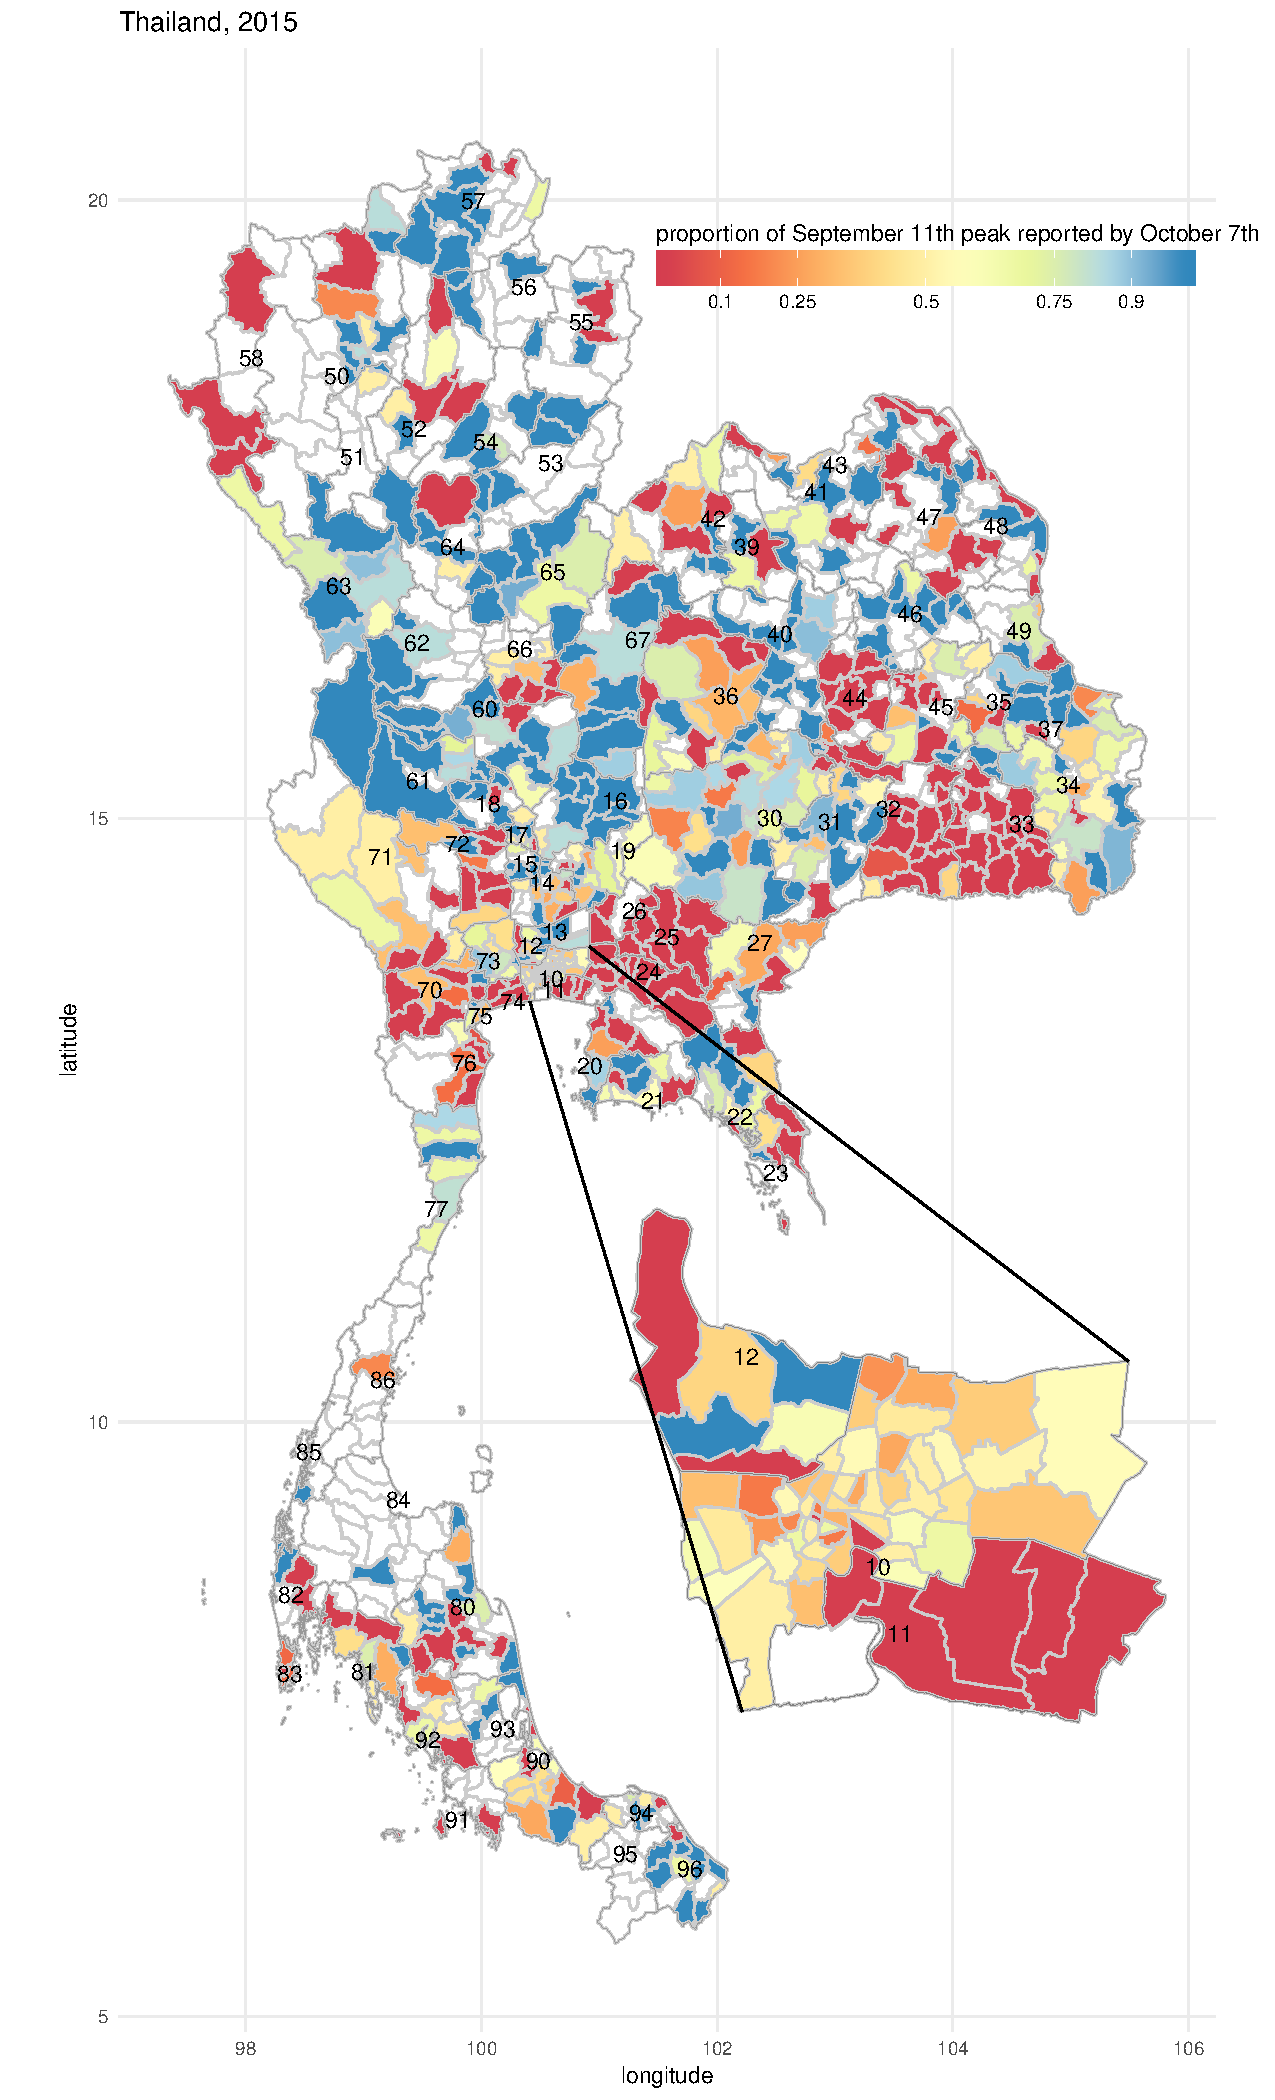
\includegraphics[width=1.0\textwidth]{thailand-ecdf-map}
 \end{center}
 \caption{\small The proportion of the 9/11 peak reported 1 month later by district is indicated by the color scale.  White districts had no cases in 2015.}
\end{figure}
\end{column}

\begin{column}{0.5\onecolwid}

\begin{block}{Hierarchical Model}
For the reporting delay data in Thailand we specify a hierarchical model for districts within provinces for the $\alpha$, $\beta$, and $q$ parameters.  There is less information available for the $\delta$ parameter so we only fit a province-level hierarchical model for $\delta$. 

\vspace{0.2in}

Each parameter is constructed through a scaled logit transform and the following model. We show the hierarchical model, for $\alpha$ only, below.  The scaling parameters are: $\kappa_\alpha=30$ $\kappa_\sigma=20$, and $\kappa_\delta=200$).

\begin{align*}
\text{logit}\left(\frac{\alpha_i}{\kappa_\alpha}\right) &= \alpha_{k[i]}   & \\
\alpha_{k} &\sim N(\alpha_{j[k]}, \sigma_{\alpha,\text{\tiny K}})    & \text{district} \\
\alpha_j &\sim N(\alpha_0, \sigma_{\alpha_\text{\tiny J}})                  & \text{province}\\
\end{align*}

Upon fitting the model we can construct an inverse CDF for any given region and produce estimates and credible intervals for the expected delay.  Currently we make predictions based on a separate simple model for counts of cases observed in district $k$ during an interval $[t_a,t_b)$ at time $t^*$ and the count of cases observed at some time $t >> t^*$.

\begin{align*}
x_{k,[t_a,t_b)}(t^*) \sim \text{Bin}(x_{k, [t_a,t_b)}(t),p_{k, [t_a,t_b)}(t^*)) \\
x_{k,[t_a,t_b)}(t) \sim \text{NB}(x_{k,[t_a,t_b)}(t^*),p_{k,[t_a,t_b)}(t^*))
\end{align*}


\end{block}
\end{column}


\end{columns}



%\begin{block}{Advantages}

%\begin{itemize}
%\item A separate parameter to describe the inflation of the (truncated) tail.  
%\item A single mixing parameter to describe the proportion of data outside of the main mass of the distribution
%\item Shape and scale parameters for the Gamma component \emph{shared} between both parts of the mixture.
%\item For simulated data drawn from a Gamma density and contaminated with the addition of very large outliers we can demonstrate improved fit for a variety of shape/scale parameters and varying amounts of contamination.
%\item Standard methods often impose censoring to deal with this issue, which requires choosing a threshold.  In our work on Thailand we have $>8,000$ administrative units with potentially different thresholds so fitting a single model is critical.
%\end{itemize}

%\end{block}

\end{column} % End of the fourth column

\begin{column}{1.3\onecolwid} 

\begin{columns}

\begin{column}{0.7\onecolwid} 

\begin{figure}
 \begin{center}
    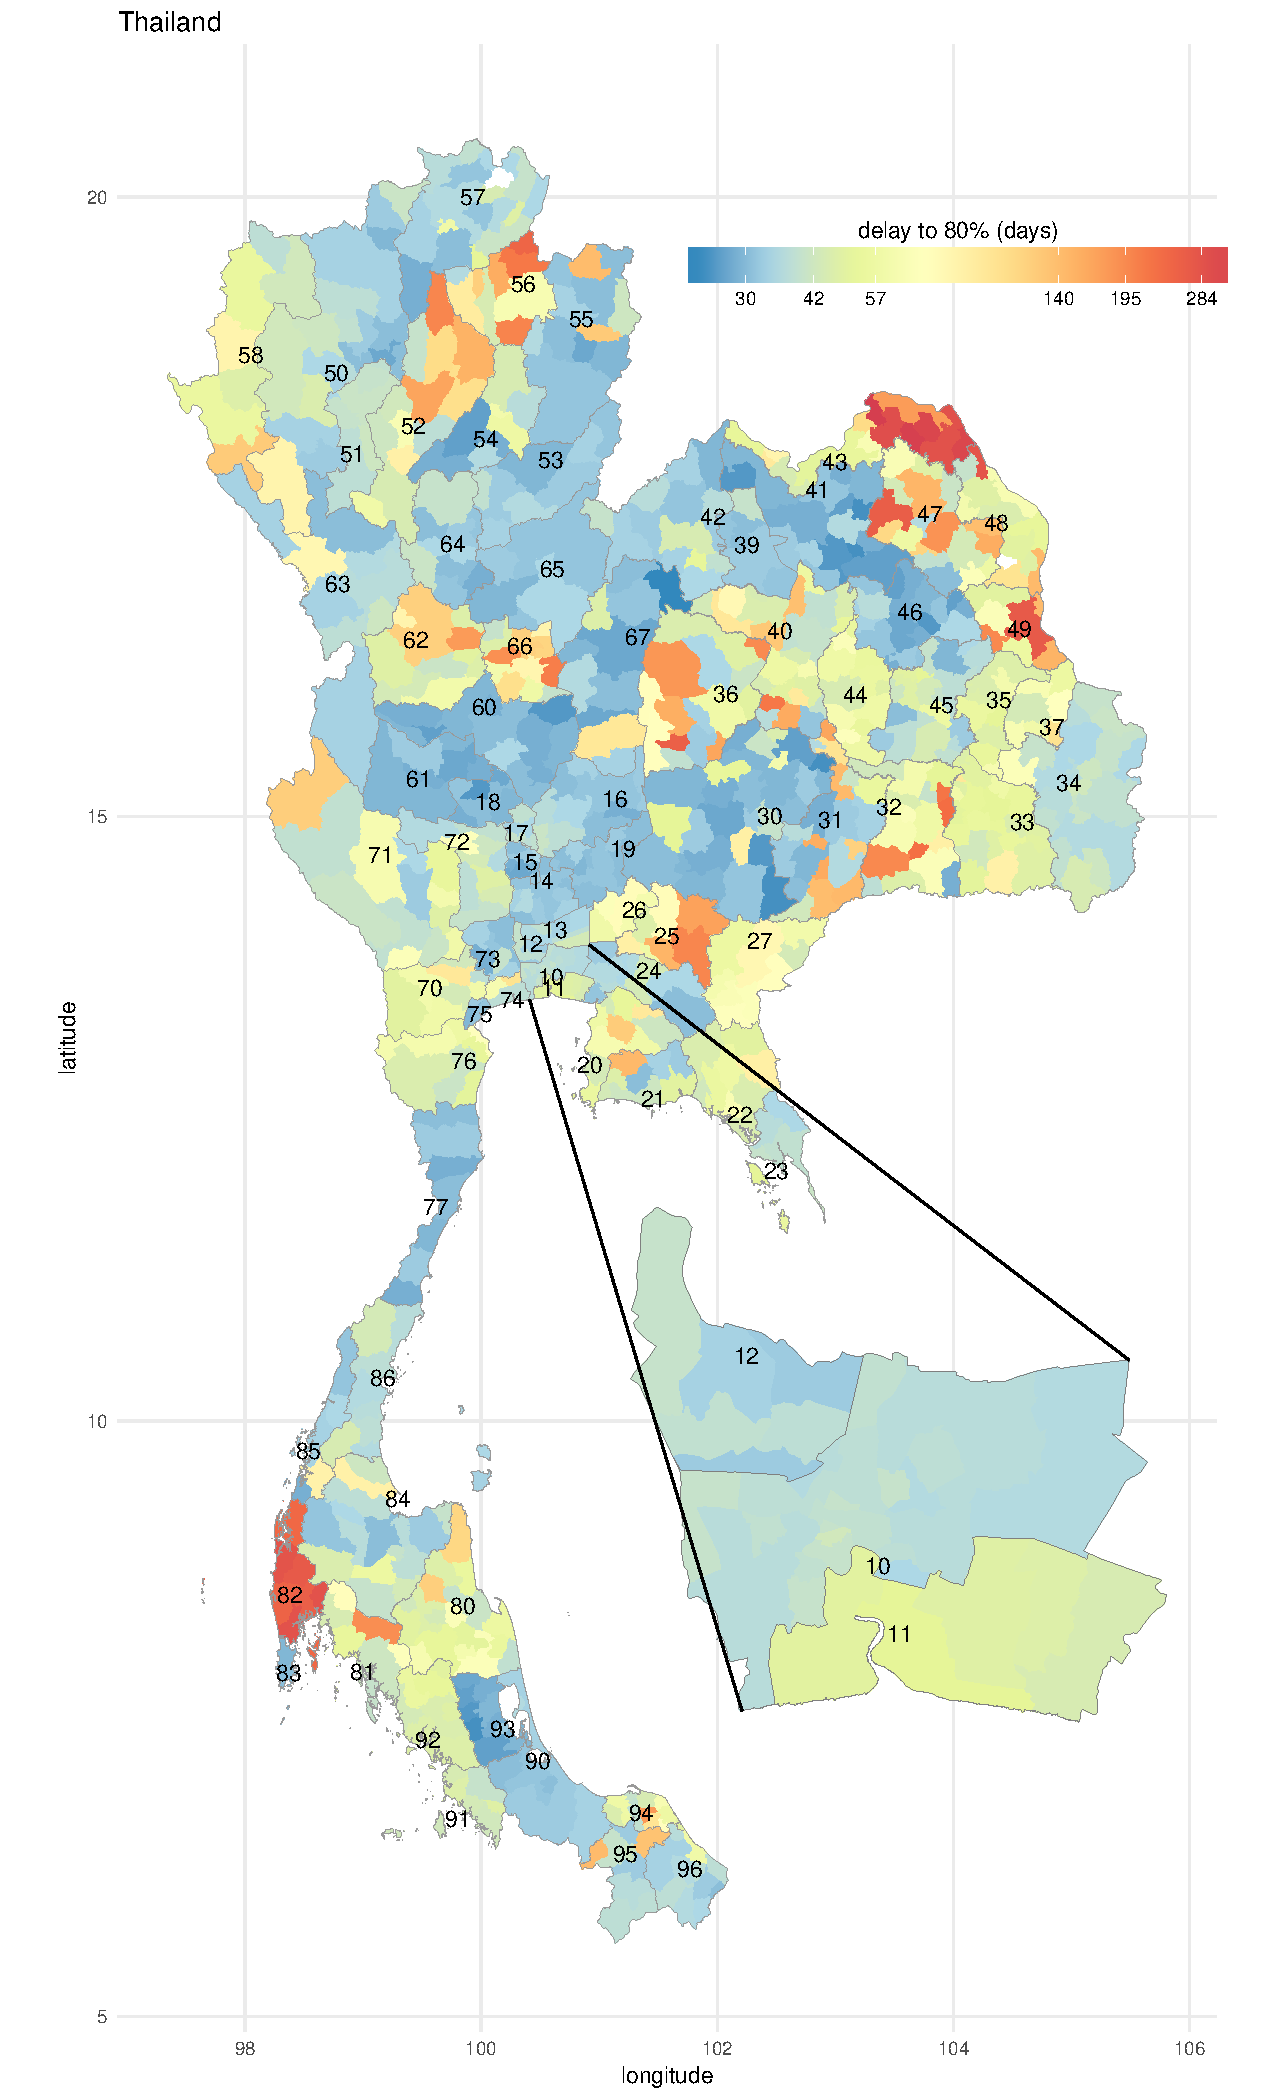
\includegraphics[width=1.0\textwidth]{thailand-model-delays}
 \end{center}
 \caption{\small The model-reconstructed time (days) it takes to report 80\% of cases by district is indicated by the color scale.}
\end{figure}

\end{column}

\begin{column}{0.6\onecolwid} 

\begin{block}{Fitting and Results}
We Stan (mc-stan.org) for programming the model as well as sampling from the posterior using an auto-tuned HMC alogrithm (NUTS).  We fit this hierarchical model to dengue reporting delay data from 2014-2016 in Thailand and produce district-level country-wide estimates of CDF and inverse CDF functions (e.g.-Figure 4).  Empirical CDF functions almost always fall within 95\% credible intervals for the estimated functions (e.g.-Figure 5) and we are working on quantifying goodness of fit.

\vspace{0.2in}

Visual examination of district-level plots reveals the hierarchical model was effective at shrinking estimates from data-sparse districts towards their province means.  The contaminated data density appears to accurately represent densities for data with marginal (1-5\%) and large (10-30\%) contamination without requiring any manual adjustments.  This was a great benefit as this version of the model covered 928 districts, and the next deeper level of data (sub-districts) includes $\sim$8,000 units making any manual adjustments prohibitive.
\end{block}

\begin{block}{Evaluation}
To evaluate the impact of this model we used it in our dengue forecasting efforts[1] to estimate true current case counts based on partially reported case counts.  \emph{We then applied the forecasting model based on the estimated true case counts and realized a $\sim$1-2 month improvement in the effective forecast horizon.} We also used a simulation study to evaluated the contaminated data density versus the generalized Gamma and Gamma densities for a variety of contaminated non-contaminated data types.  As expected our density performs well in both contexts whereas the generalized Gamma fails to fit the main mass of the density in the presence of outliers.

\end{block}


\end{column}

\end{columns}

%\begin{block}{Simulated Data Example}
%\begin{figure}
% \begin{center}
%    \includegraphics[trim={0 0cm 0 0cm}, clip, %width=1 \textwidth]{density-data-model-comparison.png}
% \end{center}
% \caption{\small Goodness of fit comparison.  %Data simulated from Gamma and either fit %directly or fit after adding Exponential (scale=50) draws to 5\% of the observations.  Models fit included the Gamma, generalized Gamma, and Gamma-Exponential Sum Gamma Mixture (GESGM)}
%\end{figure}
%\end{block}

\begin{columns}
\begin{column}{0.7\onecolwid}

\begin{figure}
 \begin{center}
    \includegraphics[width=.8\textwidth]{district-plot-126}
 \end{center}
 \caption{\small Typical match between empirical and model-based CDF for a single district.  Some districts saw few cases and are more difficult to evaluate.}
\end{figure}

\end{column}

\begin{column}{0.6\onecolwid}

\begin{block}{Ongoing Work}
This evaluation makes us confident in our ability to represent reporting delays in real-world data.  We are working to create a joint model for both reporting delays and the time-series component to realize further gains in forecasting accuracy.
\end{block}


\tiny{We would like to acknowledge the funding of NIH grant R01 AI102939-01, our Thai Ministry of Public Health collaborators for making the data available, and the efforts of the Stan development team (mc-stan.org).} \tiny{Contaminated data density and reporting model contact: Krzysztof Sakrejda, krzysztof@fawkes.io, github.com/sakrejda, Group contact: Nicholas Reich, nick@schoolph.umass.edu, reichlab.io}

\vspace{.2in}

\tiny [1] N.G. Reich et al. (2016) Challenges in Real-Time Prediction of Infectious Disease: A Case Study of Dengue in Thailand. PLoS Negl Trop Disease. 10(6):e0004761  \tiny [2] P. Effler et al. (1999) Statewide System of Electronic Notifiable Disease Reporting From Clinical Laboratories: Comparing Automated Reporting With Conventional Methods. JAMA. 282(19):1845-1850  \tiny [3] D. Revere et al. (2017) Notifiable condition reporting practices: implications for public health agency participation in a health information exchange. BMC Public Health. 17:247

\vspace{.2in}


\end{column}

\end{columns}

\end{column} 

\end{columns} % End of all the columns in the poster


\end{frame} % End of the enclosing frame
\end{document}
